\pdfminorversion=4
\documentclass[aspectratio=169]{beamer}
\usepackage[style=apa]{biblatex}
\addbibresource{2references.bib}
\useinnertheme{circles}
\newenvironment{proenv}{\only{\setbeamercolor{local structure}{fg=black}}}{}
\newenvironment{conenv}{\only{\setbeamercolor{local structure}{fg=red}}}{}
% \documentclass[9pt]{beamer}
\usetheme{Madrid}

\usepackage{movie15}
\usepackage{lmodern}
\usepackage[font=Times,timeinterval=1, timeduration=15, timedeath=0, fillcolorwarningsecond=white!60!yellow,
timewarningfirst=50,timewarningsecond=80,resetatpages=2]{tdclock}
\usepackage[scale=2]{ccicons}
\usepackage[utf8]{inputenc}
% \usepackage{apacite}
\usepackage{hyperref}
\usepackage{url}
\usepackage{helvet}
\usepackage[spanish]{babel}

\usepackage{xcolor}
\xdefinecolor{rosario}{HTML}{b31e29}
\xdefinecolor{udem}{HTML}{fee703}
\xdefinecolor{udemo}{HTML}{333333}
\xdefinecolor{udemop}{HTML}{fff500}
\xdefinecolor{cclight}{HTML}{7c0cc7}
\setbeamercolor{normal text}{fg=black}
\setbeamercolor{itemize item}{bg=yellow, fg=black}

\setbeamercolor{section in toc}{fg=rosario, bg=white}
\setbeamercolor{subsection in toc}{fg=rosario, bg=white}

\setbeamerfont{section number projected}{%
  family=\rmfamily,series=\bfseries,size=\normalsize}
  
\setbeamercolor{section number projected}{bg=rosario,fg=white}
\setbeamercolor{subsection number projected}{bg=rosario,fg=white}

\setbeamercolor{background canvas}{bg=white}
\setbeamercolor{frametitle}{fg=white, bg=rosario}
\setbeamercolor{block title}{bg=rosario,fg=white}
\setbeamercolor{block body}{bg=pink,fg=black}
\setbeamercolor{itemize item}{fg=black}
\setbeamercolor{navigation symbols}{bg=udemo,fg=udemo}

\setbeamercolor{title}{fg=white, bg=rosario}
\setbeamercolor{author}{fg=udemo}
\setbeamercolor{institute}{fg=udemo}
\setbeamercolor{titlelike}{fg=black, bg=gray}

\setbeamercolor*{palette primary}{bg=rosario,fg=white}
\setbeamercolor*{palette secondary}{bg=rosario,fg=white}
\setbeamercolor*{palette tertiary}{bg=rosario,fg=white}


\usepackage{tikz}
\usepackage{kantlipsum}

\setbeamercolor{normal text}{fg=black}
% \setbeamertemplate{background}{\tikz[overlay,remember picture]\node[opacity=.2]at (current page.center){\includegraphics[width=6.7cm]{udem.png}};}

\setbeamercolor{bibliography entry author}{fg=black}
\setbeamercolor{bibliography entry title}{fg=black}
\setbeamercolor{bibliography entry location}{fg=black}
\setbeamercolor{bibliography entry note}{fg=black}
\setbeamercolor{itemize item}{fg=black}

\setbeamertemplate{bibliography item}{}

\title[Analítica para Proyectos]{Analítica para Proyectos}
% \subtitle{(Reflexiones para colegas)}
% \date{}
\author[Juan C. Correa (\url{https://correajc.com/})]{Prof. Juan C. Correa, Ph.D.\href{https://orcid.org/0000-0002-0301-5641}{
\includegraphics[width=0.3cm]{orcid.png}}}

\institute[]{Maestría en Estructuración Ágil de Proyectos de Alta Complejidad\\
Universidad del Rosario\\
\Email  \href{mailto:juanca.correa@urosario.edu.co}{\color{blue}juanca.correa@urosario.edu.co}
}

\pgfdeclareimage[height=1cm]{UR}{UR}
 \logo{\pgfuseimage{UR}}
 \setbeamertemplate{caption}[numbered]
\date[\initclock
\quad\cronominutes\pdfcolon\cronoseconds ~~Bogotá, Abril 11, 2024] % (optional)
{}

\subject{}


\begin{document}
% \end{document}
\frame{\titlepage}

\begin{frame}{Plan de Evaluación}
\begin{figure}
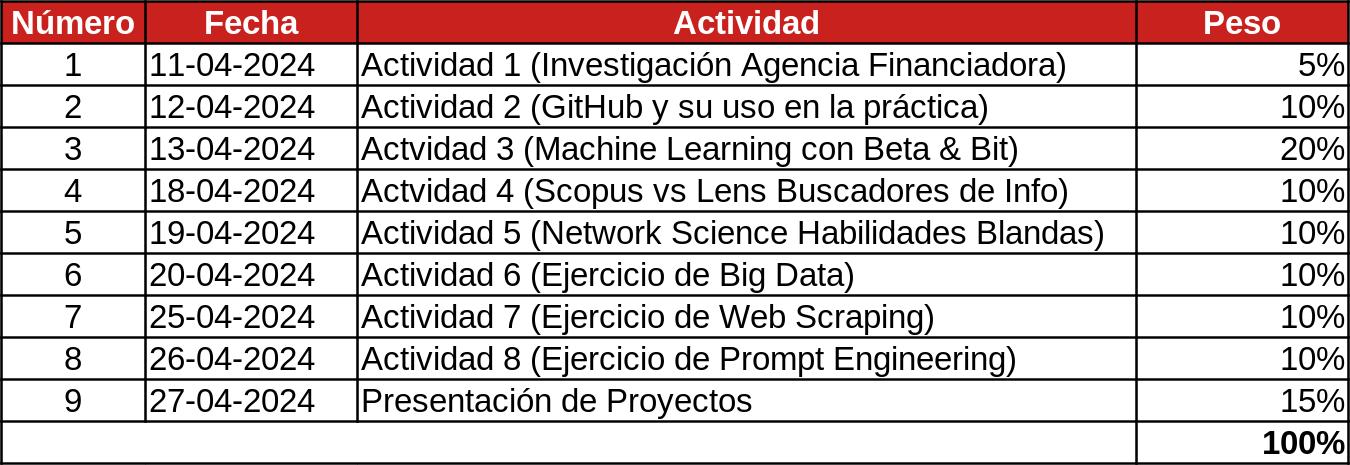
\includegraphics[width=.9\textwidth]{evaluaciones.png}
\end{figure}   
\end{frame}

\begin{frame}{Plan de Evaluación}
La entrega del proyecto final debe reunir lo siguiente
\begin{itemize}
\item[1.]  Una presentación orientada a resolver un problema local, regional, o global.
\item[2.] Un repo de GitHub para evidenciar el desarrollo tecnológico en el que se apoya la solución planteada (cualquiera de los planteados en actividades 3,5,6,7, u 8).
\item[3.] La literatura técnica que respalda la solución tecnológica.
\item[4.] Un pitch de 3 minutos para captar el interés de la agencia financiadora 
\item[5.] Máximo número de participantes por equipo: 2  
\item[6.] Un capítulo para el siguiente \href{https://apgpac.netlify.app/}{\textcolor{blue}{e-book}}, siguiendo las instrucciones de la próxima clase.
\end{itemize}
\end{frame}



\begin{frame}
\begin{block}{Al finalizar esta clase, usted va a conocer:}
\vspace{.2cm}
\begin{itemize}
\item[\textcolor{ccdark}{1}] Por qué es necesario hablar de analítica para los proyectos. 
\vspace{.2cm}
\item[\textcolor{ccdark}{2}] Por qué hay urgencia de abordar proyectos con gran impacto.
\vspace{.2cm}
\item[\textcolor{ccdark}{3}] El ecosistema de tecnologías que aceleran los proyectos.
\vspace{.2cm}
\item[\textcolor{ccdark}{4}] Entender los desafíos de acelerar la gestión de proyectos.
\end{itemize}    
\end{block}
\end{frame}


\setbeamertemplate{background}{\tikz[overlay,remember picture]\node[opacity=0.2]at (current page.center){\includegraphics[width=13cm]{}};}

\begin{frame}
\frametitle{~~~~~~~~~~~~~~~~~~~~~~~~~~~~~~~~~~~~~~~~~~~~~~~~~~~~~~~~~~~~~~~~~~~~~~~~~~~~~~~~~~~~~~~~~~~~~~~~~~~Contenidos} 
\tableofcontents
\end{frame}


\setbeamertemplate{background}{\tikz[overlay,remember picture]\node[opacity=0.8]at (current page.center){\includegraphics[width=17cm]{}};}
\section{¿Por qué hablar de analítica para los proyectos?}
\begin{frame}
\initclock
\centering
\Huge
¿Por qué hablar sobre\\
analítica para los proyectos?\\
\vspace{2cm}
\end{frame}

\begin{frame}
\huge{Porque el uso del conocimiento útil no solo ocurre en la universidad, sino también en las empresas y en el gobierno y su utilidad depende de nuestros valores éticos.}    
\end{frame}

\begin{frame}
\begin{columns}
\begin{column}{0.5\textwidth}
\begin{figure}
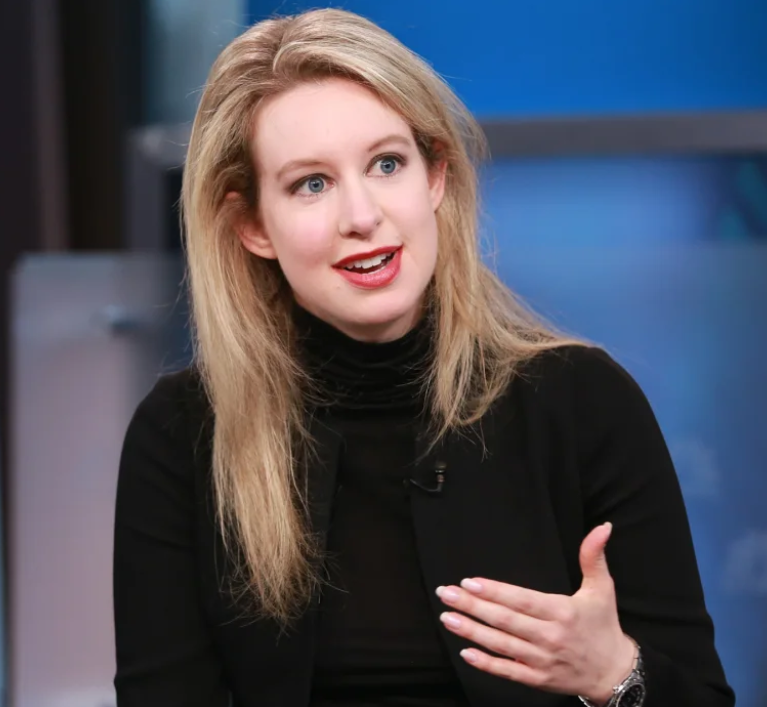
\includegraphics[width=.6\textwidth]{Holmes.png}
\end{figure}   
\end{column}
\begin{column}{0.5\textwidth}
Elizabeth Holmes (Fundó Theranos con una primera ronda de inversión que recaudó 700 millones de dólares por filántropos interesados en su propuesta. En el momento más cumbre, su empresa alcanzó una valoración de 10 mil millones de dólares sobre innovaciones fraudulentas sin respaldo científico comprobado).\\

\end{column}
\end{columns}
\end{frame}

\begin{frame}
\begin{columns}
\begin{column}{0.5\textwidth}
\begin{figure}

\includegraphics[width=.6\textwidth]{Ruja.png}
\end{figure}   
\end{column}
\begin{column}{0.5\textwidth}
Ruja Ignatova (Fundó OneCoin una corporación orientada al desarrollo de una criptomoneda descentralizada con mejores propiedades que BitCoin, resultando ser una organización de marketing y ventas piramidal estafando a más de 3 millones de ``clientes'' por una cifra cercana a los 4.037 millones de dólares).
\end{column}
\end{columns}
\end{frame}

\begin{frame}
\begin{columns}
\begin{column}{0.5\textwidth}
\begin{figure}
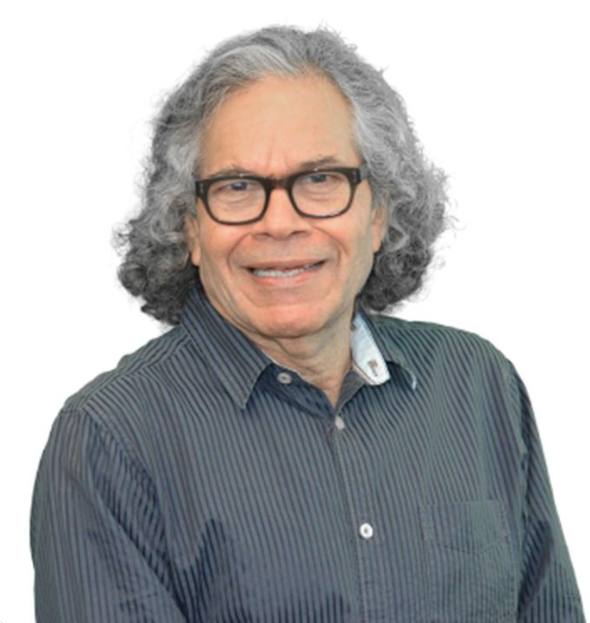
\includegraphics[width=.8\textwidth]{Kapoor.png}
\end{figure}   
\end{column}
\begin{column}{0.5\textwidth}
John Kapoor (Fundó Insys Therapeutics, la principal productora de fentanilo, un potente opiode liberador del dolor para pacientes crónicos con cáncer. El fentanilo adquirió popularidad debido a que la compañía tenía la práctica de sobornar a médicos profesionales para que actuaran como ``promotores'' del medicamento incluyendo a pacientes sin cáncer).
\end{column}
\end{columns}
\end{frame}



\begin{frame}
\begin{columns}
\begin{column}{0.5\textwidth}
Richard Stallman (Creador de la Fundación para el Software Libre, la licencia de protección de propiedad intelectual libre y el sistema operativo GNU que fue la base fundamental del sistema operativo Linux).\\
\end{column}
\begin{column}{0.5\textwidth}
\begin{figure}
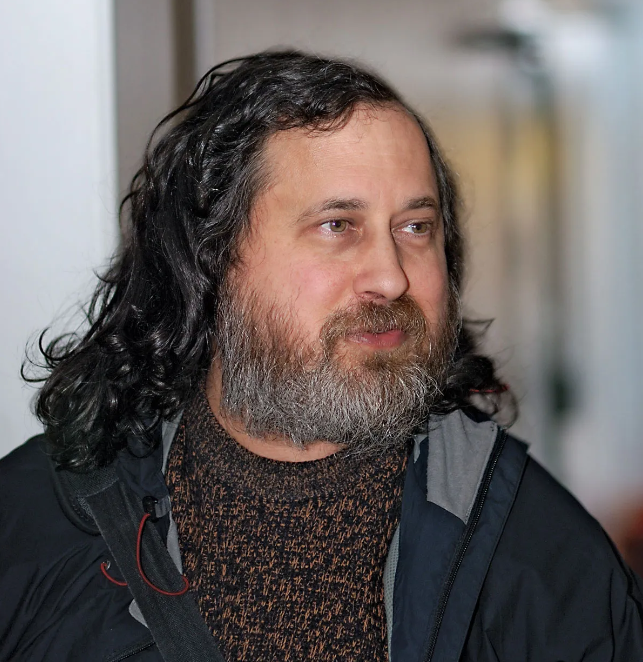
\includegraphics[width=.6\textwidth]{Stallman.png}
\end{figure}   
\end{column}
\end{columns}
\end{frame}

\begin{frame}
\begin{columns}
\begin{column}{0.5\textwidth}
Linus Torvalds (Creador de Git una aplicación para la gestión de versiones en desarrollo de software, y el Kernel Linux, base del sistema operativo Linux y dispositivos Android y en todos los servidores de grandes instituciones públicas y privadas mundialmente).\\
\end{column}
\begin{column}{0.5\textwidth}
\begin{figure}
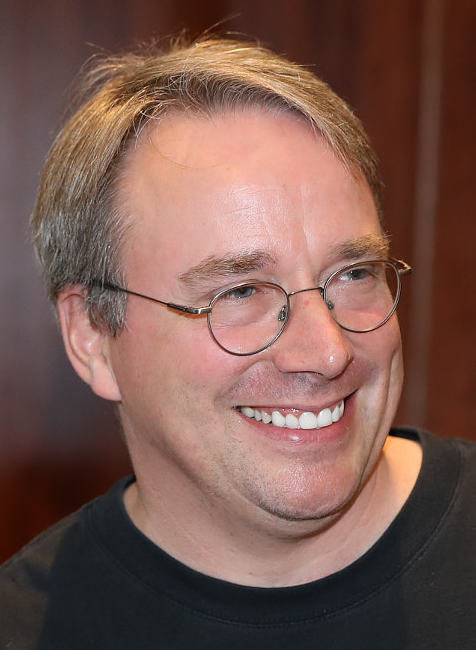
\includegraphics[width=.5\textwidth]{Linus.jpeg}
\end{figure}   
\end{column}
\end{columns}
\end{frame}

\begin{frame}
\begin{columns}
\begin{column}{0.5\textwidth}
Guido van Rossum (Creador del lenguaje de programación Python; un lenguaje de programación fundamental para el desarrollo de productos y servicios tan diversos como Ansible, Airbnb, Spotify, Instagram, Pinterest, Reddit, Amazon, Alexa, TensorFlow, PyTorch, Scikit-learn, además de video-juegos ).\\
\end{column}
\begin{column}{0.5\textwidth}
\begin{figure}
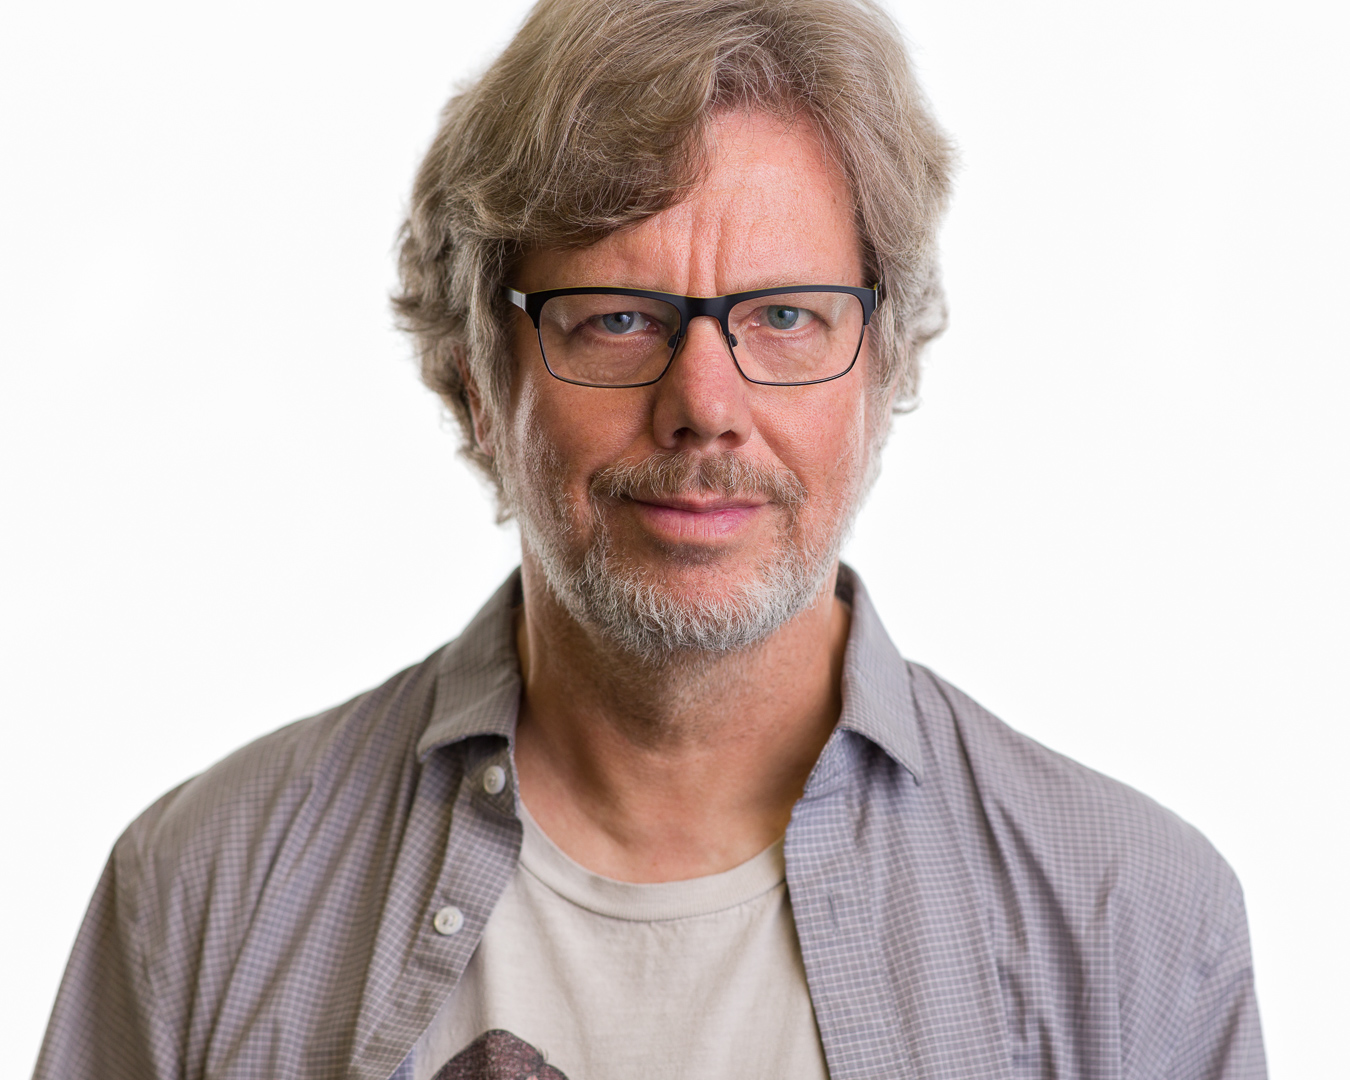
\includegraphics[width=.8\textwidth]{Guido.jpg}
\end{figure}   
\end{column}
\end{columns}
\end{frame}

\begin{frame}
\begin{columns}
\begin{column}{0.5\textwidth}
Rafael Reif (Rector del MIT entre 2012 y 2022, único latino (venezolano) en llegar a ocupar la máxima posición de liderazgo en una de las mejores universidades de fuerte tradición científica en USA. Su campaña ``\textbf{Better World}'' fue un éxito sin precedentes al captar \textbf{6.24 mil millones de dolares} para estimular la innovación dirigida a desafíos globales).\\
\end{column}
\begin{column}{0.5\textwidth}
\begin{figure}
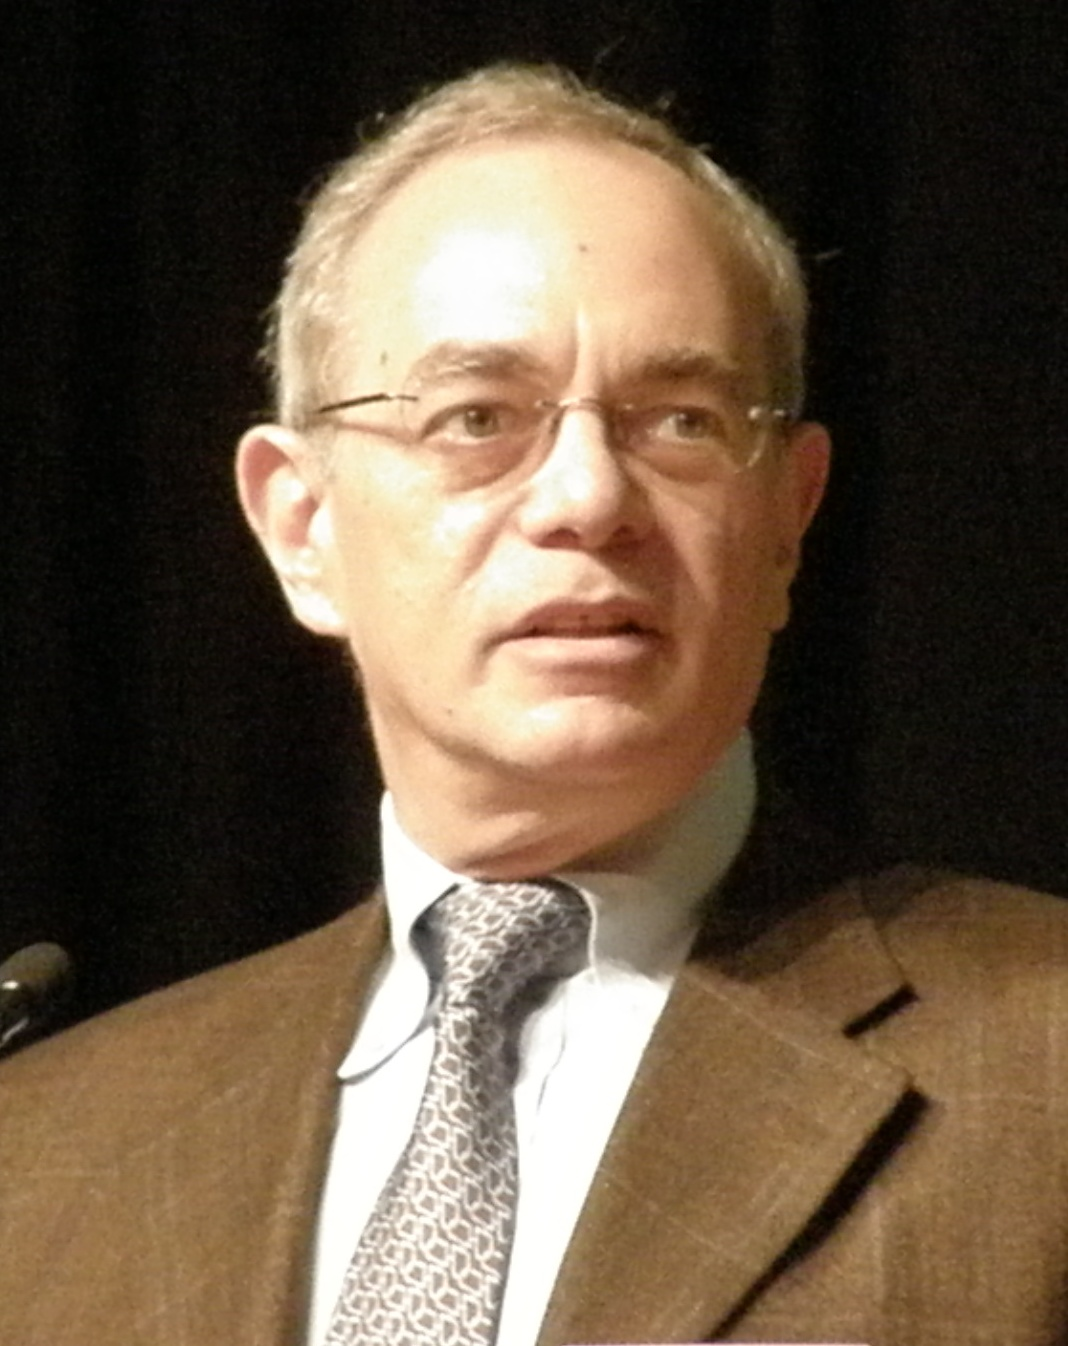
\includegraphics[width=.6\textwidth]{Reif.jpg}
\end{figure}   
\end{column}
\end{columns}
\end{frame}

\begin{frame}
El Atlas de Complejidad Económica muestra un caso exitoso de triple hélice desarrollado inicialmente por \textcite{hidalgo2009}.
\begin{figure}
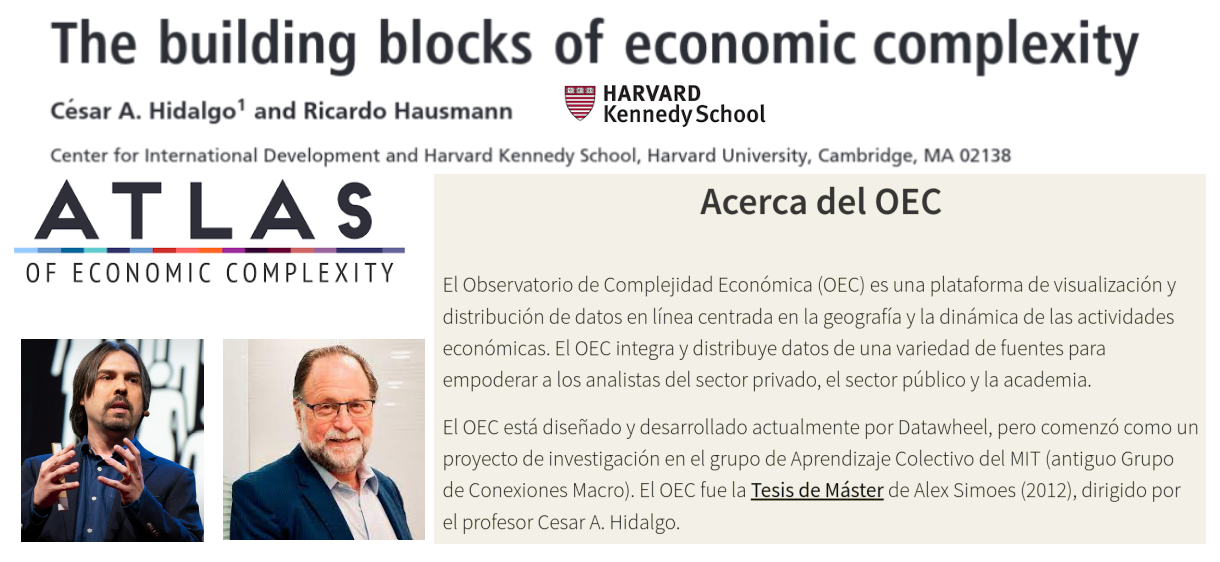
\includegraphics[width=.7\textwidth]{Atlas.png}
\end{figure}
\end{frame}


\begin{frame}
\begin{figure}
\centering
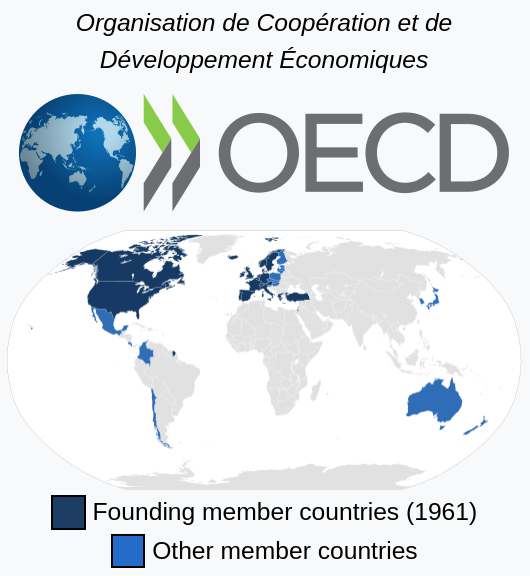
\includegraphics[width=0.45\textwidth]{oecd.png}
\end{figure}
\end{frame} 

\begin{frame}
\url{https://data.oecd.org/eduatt/population-with-tertiary-education.htm}
\begin{figure}
\centering
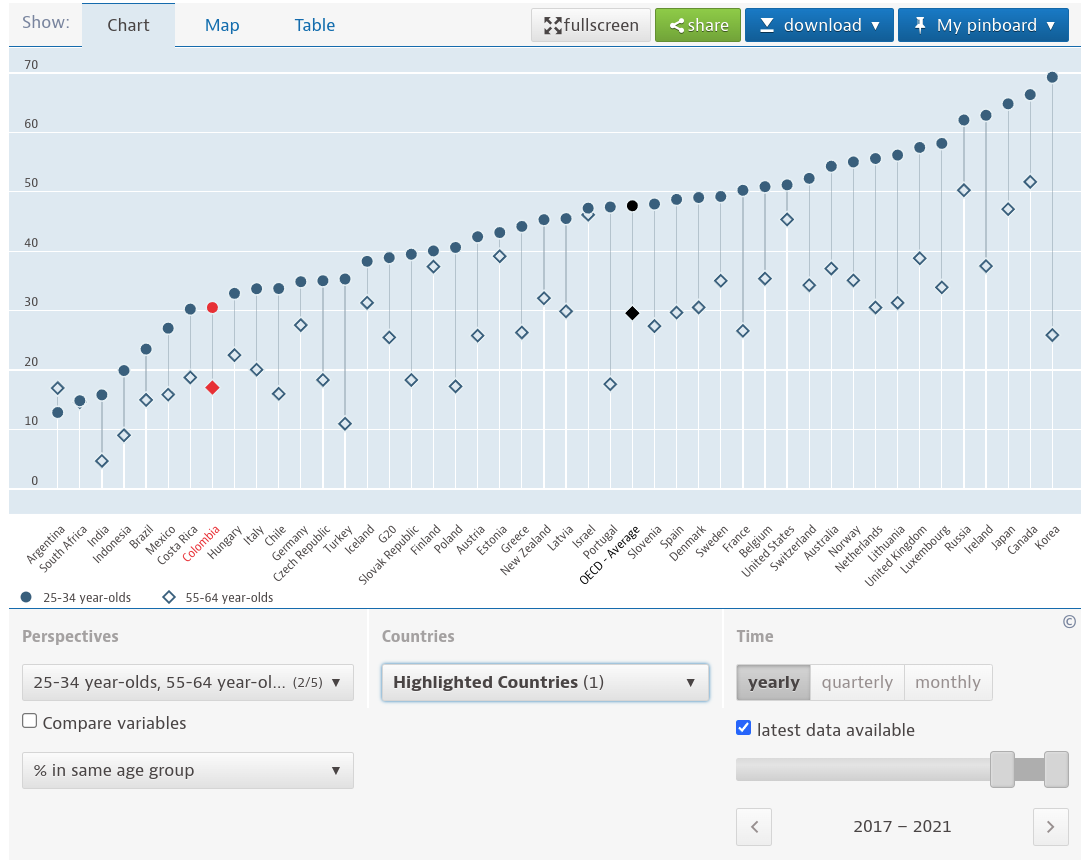
\includegraphics[width=0.6\textwidth]{OECD3.png}
\end{figure}
\end{frame} 

\begin{frame}
\begin{figure}
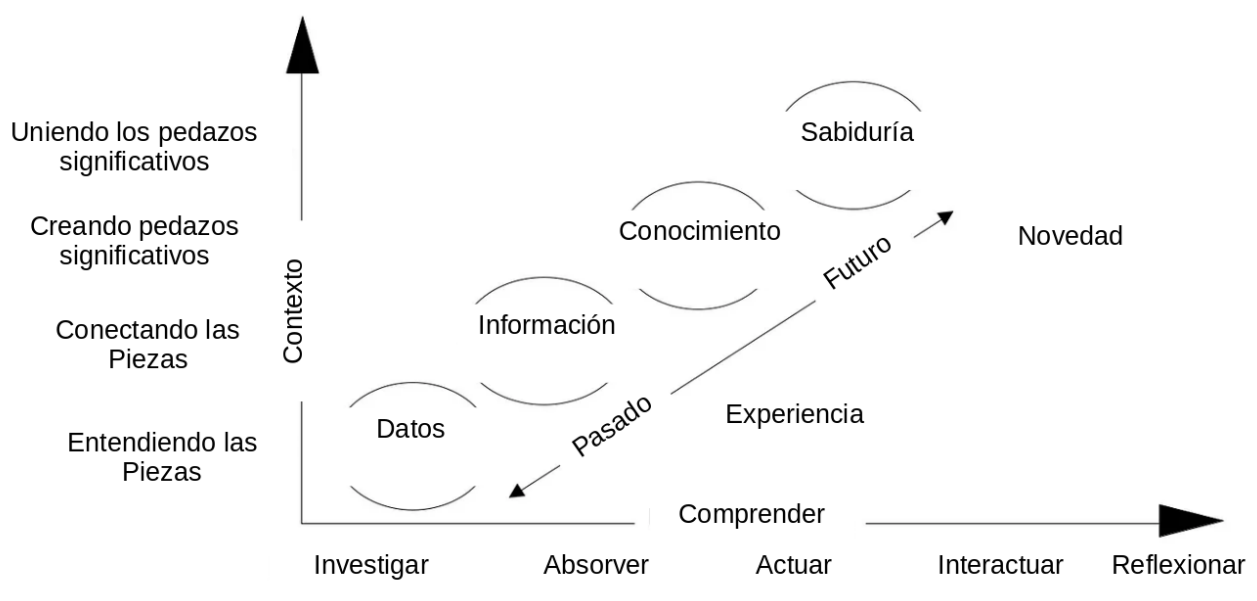
\includegraphics[width=.95\textwidth]{jerarquia.png}
\end{figure}       
\end{frame}

\subsection{Una Experiencia en Bogotá}

\begin{frame}
\begin{figure}
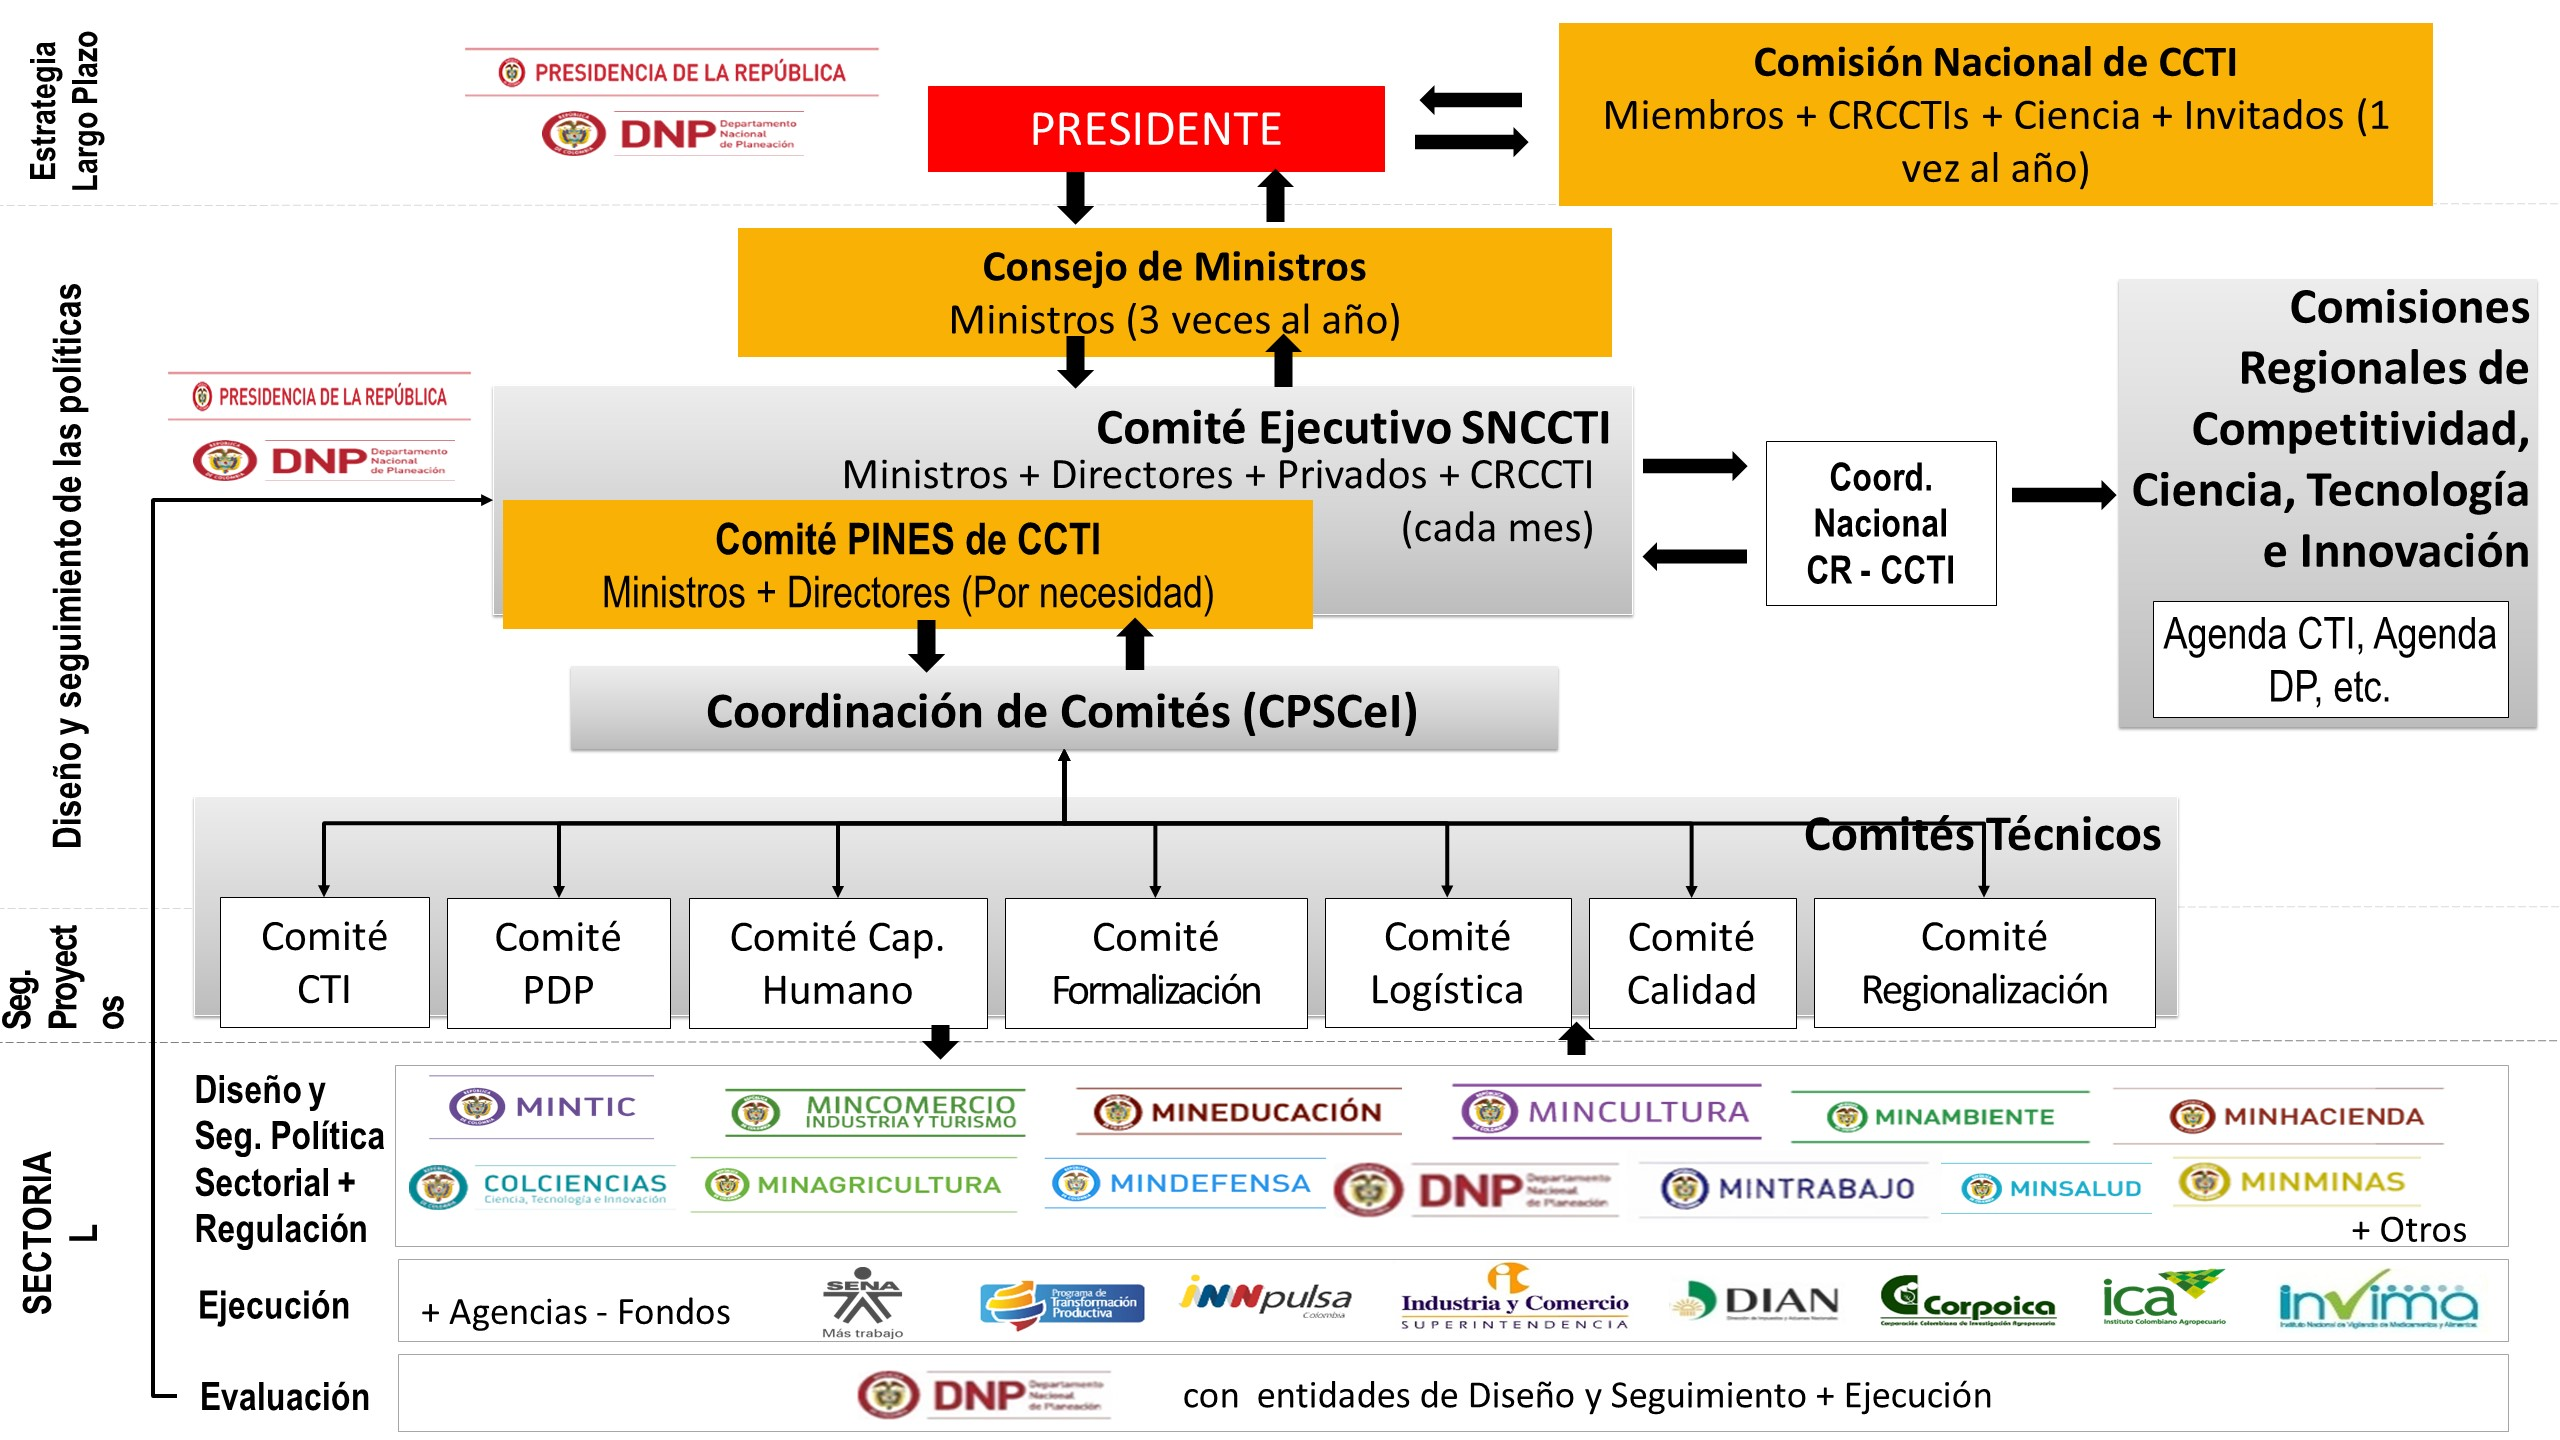
\includegraphics[width=.85\textwidth]{diagrama.jpg}
\end{figure}       
\end{frame}

\setbeamertemplate{background}{\tikz[overlay,remember picture]\node[opacity=1]at (current page.center){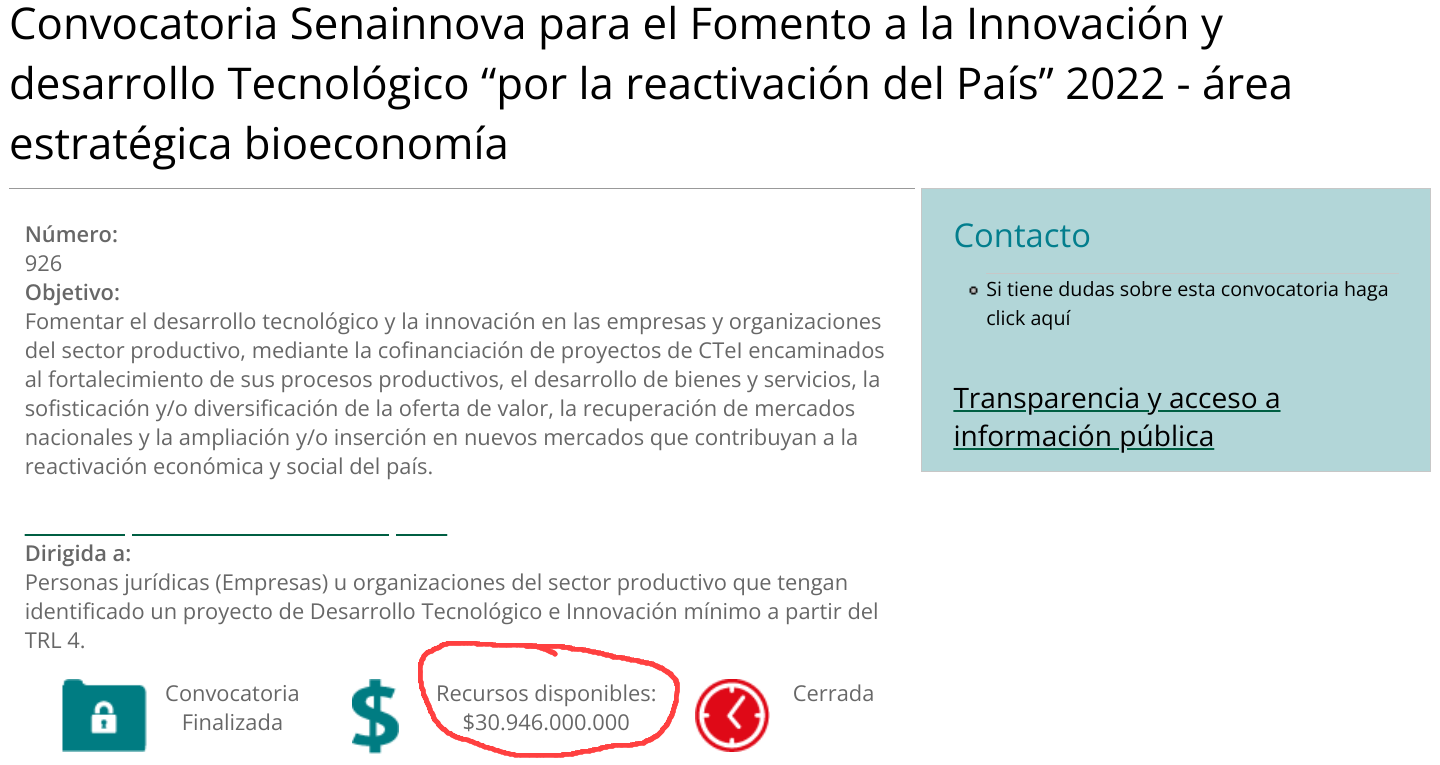
\includegraphics[width=15cm]{SenaInnova.png}};}
\begin{frame}
\end{frame}

\setbeamertemplate{background}{\tikz[overlay,remember picture]\node[opacity=1]at (current page.center){
\includegraphics[width=15cm]{Triple.png}};}
\begin{frame}
\end{frame}

\setbeamertemplate{background}{\tikz[overlay,remember picture]\node[opacity=1]at (current page.center){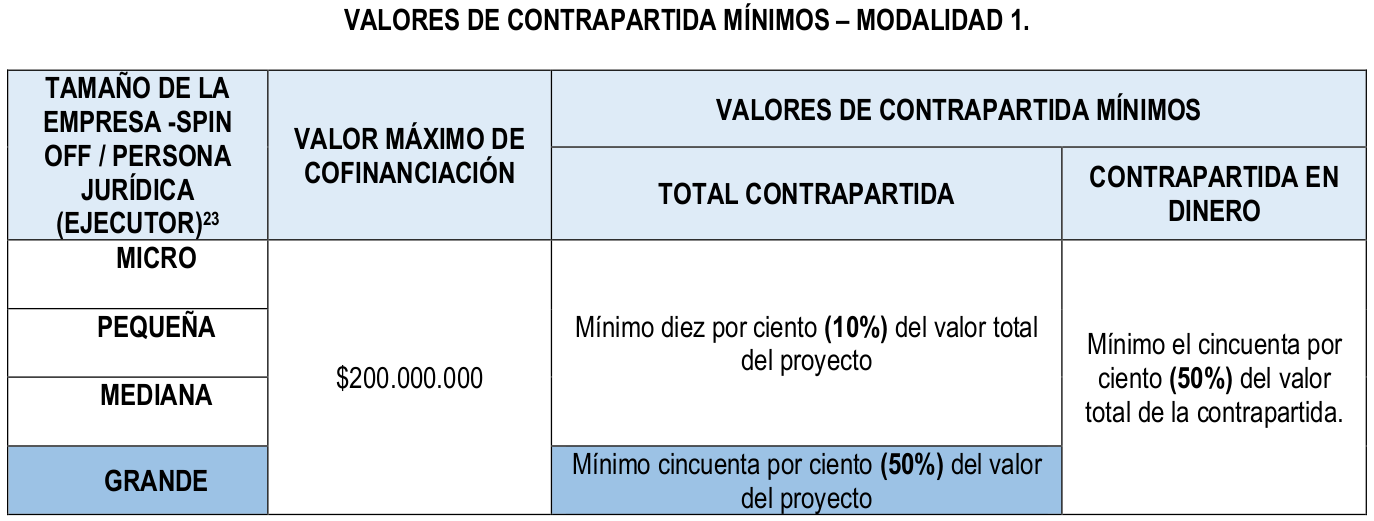
\includegraphics[width=14cm]{Modalidad1.png}};}
\begin{frame}
\end{frame}

\setbeamertemplate{background}{\tikz[overlay,remember picture]\node[opacity=1]at (current page.center){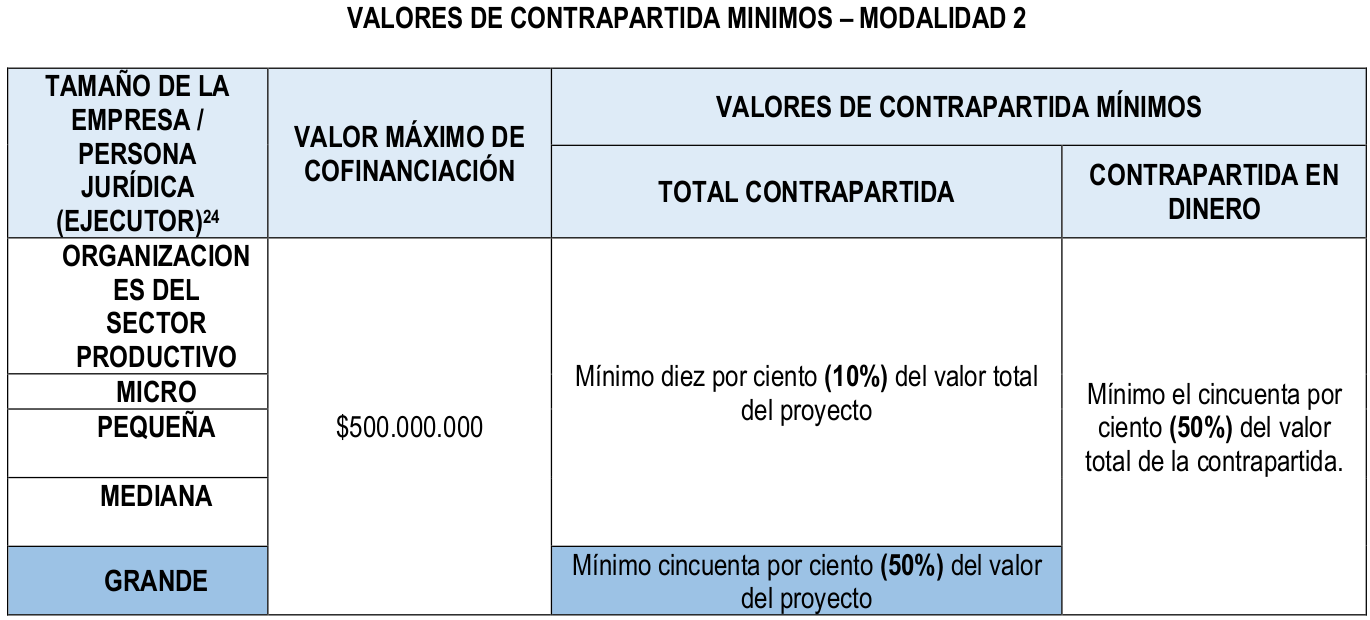
\includegraphics[width=14cm]{Modalidad2.png}};}
\begin{frame}
\end{frame}




\section{La Urgencia de Proyectos con Impacto}

\setbeamertemplate{background}{\tikz[overlay,remember picture]\node[opacity=1]at (current page.center){\includegraphics[width=14cm]{}};}
\begin{frame}
\centering
\Huge
La Urgencia de Proyectos con Impacto
\end{frame}

\setbeamertemplate{background}{\tikz[overlay,remember picture]\node[opacity=1]at (current page.center){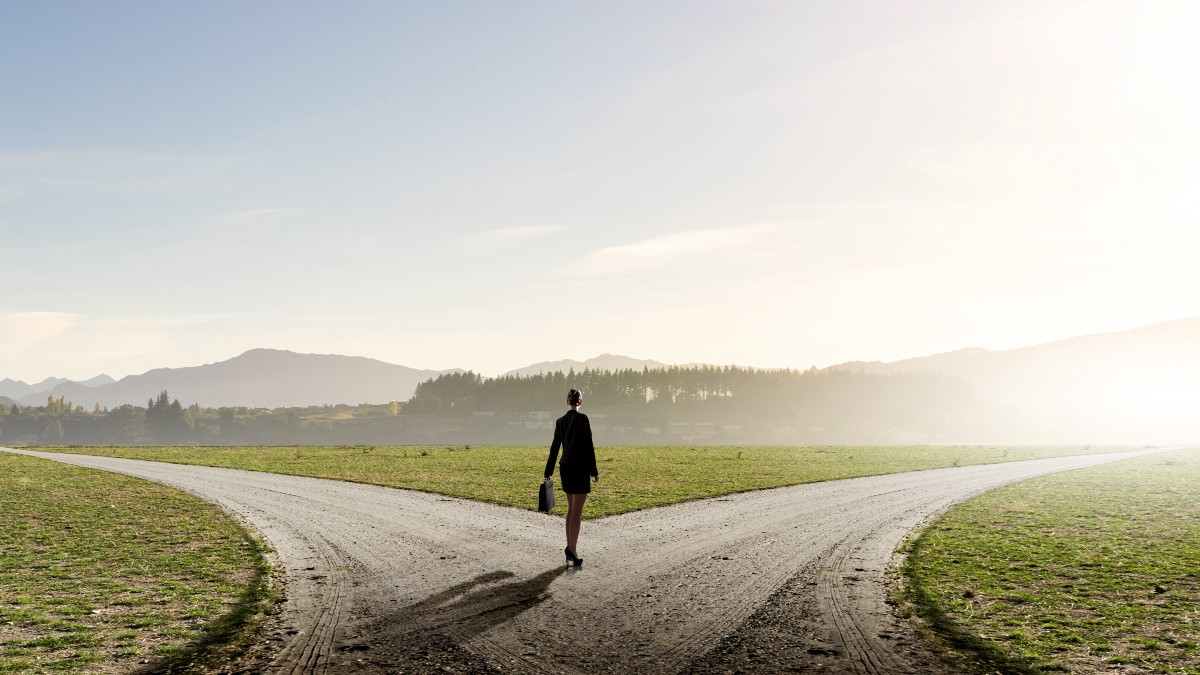
\includegraphics[width=16cm]{TwoWays.jpeg}};}

\begin{frame}
\huge
\centering
¿Qué opción escoges para ``garantizar'' la continuidad de la vida humana?\\
% \vspace{6.5cm}
\begin{columns}
\begin{column}{0.5\textwidth}
\begin{figure}

\includegraphics[width=.35\textwidth]{QR_adaptarnos.png}
\end{figure}   
\end{column}
\begin{column}{0.5\textwidth}
\begin{figure}

\includegraphics[width=.35\textwidth]{QR_revertir.png}
\end{figure}   
\end{column}
\end{columns}
\end{frame}

\begin{frame}
\centering
Actividad de Discusión\\
(15 minutos)
\begin{columns}
\begin{column}{0.5\textwidth}
\begin{figure}
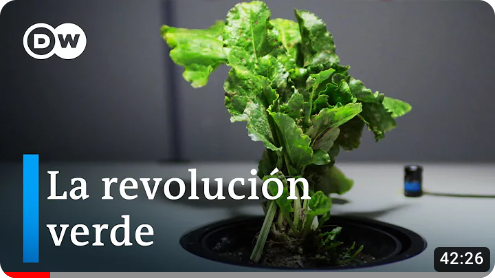
\includegraphics[width=.55\textwidth]{verde.png}
\end{figure}   
\end{column}
\begin{column}{0.5\textwidth}
\begin{figure}
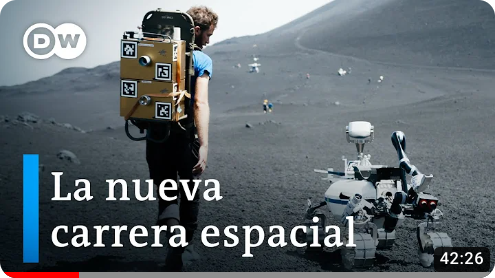
\includegraphics[width=.55\textwidth]{negro.png}
\end{figure}   
\end{column}
\end{columns}
\end{frame}

\setbeamertemplate{background}{\tikz[overlay,remember picture]\node[opacity=1]at (current page.center){\includegraphics[width=16cm]{}};}

\subsection{Actividad Evaluada 1}
\begin{frame}{Actividad Evaluada 1}
\centering
En 30 minutos vamos a investigar sobre alguna institución pública o privada dispuesta a otorgar dinero para proyectos que ``garantizan'' la continuidad de la vida humana.\\
% \vspace{1cm}
\begin{figure}

\includegraphics[width=.2\textwidth]{ActEvaluada.png}
\end{figure}
Al terminar, escanea el QR y llena este formulario.
\end{frame}

\section{Ecosistema de Tecnologías}
\setbeamertemplate{background}{\tikz[overlay,remember picture]\node[opacity=1]at (current page.center){\includegraphics[width=16cm]{}};}
\begin{frame}
\centering
\Huge
Ecosistema Tecnológico
\end{frame}


\begin{frame}
\begin{figure}

\includegraphics[width=1\textwidth]{Ecosistema.png}
\end{figure}    
\end{frame}


\section{Desafíos sobre la Gestión de Proyectos}



\begin{frame}[allowframebreaks]{Referencias}
\printbibliography[heading=none]
\end{frame}

\end{document}